% Created by tikzDevice version 0.12.3.1 on 2022-01-16 03:38:15
% !TEX encoding = UTF-8 Unicode
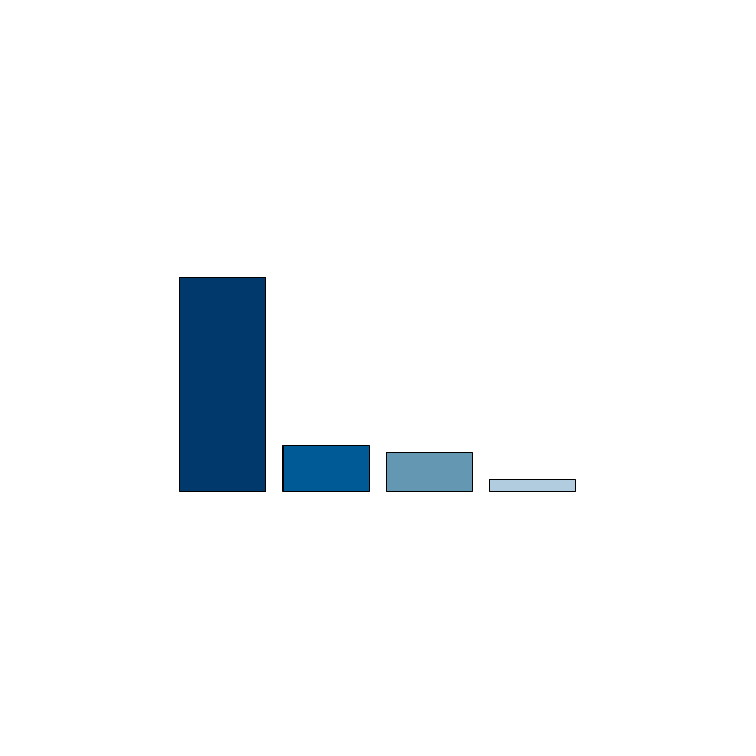
\begin{tikzpicture}[x=1pt,y=1pt]
\definecolor{fillColor}{RGB}{255,255,255}
\path[use as bounding box,fill=fillColor,fill opacity=0.00] (0,0) rectangle (252.94,252.94);
\begin{scope}
\path[clip] (  0.00,  0.00) rectangle (252.94,252.94);
\definecolor{drawColor}{RGB}{0,0,0}
\definecolor{fillColor}{RGB}{2,57,108}

\path[draw=drawColor,line width= 0.4pt,line join=round,line cap=round,fill=fillColor] ( 54.92, 85.20) rectangle ( 86.03,162.82);
\definecolor{fillColor}{RGB}{0,90,150}

\path[draw=drawColor,line width= 0.4pt,line join=round,line cap=round,fill=fillColor] ( 92.25, 85.20) rectangle (123.36,101.93);
\definecolor{fillColor}{RGB}{100,151,177}

\path[draw=drawColor,line width= 0.4pt,line join=round,line cap=round,fill=fillColor] (129.58, 85.20) rectangle (160.69, 99.31);
\definecolor{fillColor}{RGB}{178,204,223}

\path[draw=drawColor,line width= 0.4pt,line join=round,line cap=round,fill=fillColor] (166.91, 85.20) rectangle (198.02, 89.64);
\end{scope}
\end{tikzpicture}
